\chapter{Framework Application}
\label{chapter:application}

To verify that the final version of the framework was effective (see Chapter~\ref{chapter:framework}), I applied it to design a place photo discovery application as well as to reevaluate five of the applications that were used in the construction of the preliminary framework described in Chapter~\ref{chapter:old_framework}. This section outlines application design process, and evaluations of the tools with proposed directions for development of these applications. 

{\section{Design Process}

}%end section

{\section{KeePlaces}
\begin{figure}[ht!]
	\noindent
	\centering
	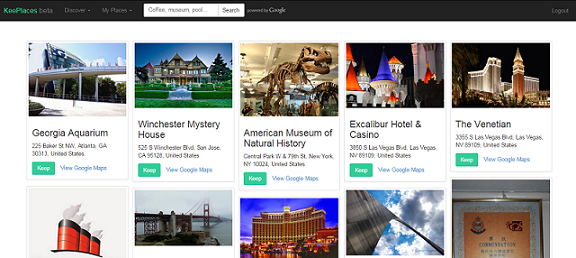
\includegraphics[width=\linewidth]{keeplaces.png}
	\caption{KeePlaces}
	\label{fig:keeplaces} 
\end{figure}
{\subsection{Navigation}
Descriptional navigation is possible using search. The search feature is not guided, and so far, results are not personalized. 

}
{\subsection{Exploration}
Spatial exploration of multiple resources is enabled through the gallery view. 
Resources are represented as photos, so visual exploration of multiple resources is enabled. However, there is no way of exploring each resource individually, therefore, exploration of a single resource is not supported. 
}
{\subsection{Integration}
KeePlaces is integrated with Google Maps.
}
{\subsection{Curation}
Curation in Keeplaces is supported through management and preservation.

Management is implemented using collection-based classification.
Every photo discovered on the site can be bookmarked, or 'kept', in a collection.
}
{\subsection{Channeling}
Channeling has not yet been enabled within the application, but it is an important aspect behind the conceptual model of the application.
}
{\subsection{Directions for Future Development}
As mentioned above, channeling is the first aspect that needs to be implemented along with enhancing management mechanisms.
}
} % end section




